\chapter{Cluster decay in $^{294}$Og}\label{chap:294Og}

\section{Cluster emission in Superheavy Elements}

The region of superheavy elements (Z>104) is an interesting one for the study of spontaneous fission because the liquid drop model predicts that all isotopes with Z>104 are unstable with respect to spontaneous fission. These nuclei are stabilized due to shell effects, but they nevertheless remain short-lived and many of them will decay by spontaneous fission regardless.

Experimentally, spontaneous fission has been observed from several superhavy isotopes (see the right panel of Figure \ref{fig:karpovshedecay}). Other observed SHEs undergo a series of alpha decays, which chains terminate in spontaneous fission. Furthermore, a variety of models predict regions of spontaneous fission in the superheavy regime. One example is shown in Figure \ref{fig:karpovshedecay}, in which lifetimes were computed for several types of decays using empirical formulas and the results compared to estimate branching ratios. Figure \ref{fig:warda2012she} is similar, except that the spontaneous fission lifetimes were computed microscopically, as were the $Q_\alpha$ values used to estimate alpha decay lifetimes.


\begin{figure}
	\centering
	\includegraphics[width=0.9\linewidth]{TeX_files/294Og_Karpov_SHEdecay}
	\caption[Calculated and experimental decay modes for SHE]{Calculated (left) and experimental (right) decay modes for SHE, based on an analysis of lifetimes calculated via emprical formulae. The boxed isotopes in the left panel are those which have been measured experimentally. Isotopes falling inside the 1$\mu$s contour are predicted to live longer than 1$\mu$s. Figure adapted from \cite{Karpova}.}
	\label{fig:karpovshedecay}
\end{figure}


\begin{figure}
	\centering
	\includegraphics[width=0.7\linewidth]{TeX_files/294Og_Warda2012_SHE}
	\caption[Dominant decay modes for SHE in a nuclear DFT-based framework.]{Dominant decay modes for SHE in a nuclear DFT-based framework are indicated. The label "RS" stands for "reflection symmetric" and "NRS" stands for "non-reflection symmetric." The colorbar indicates the predicted half-life on a logarithmic scale. Figure from \cite{Warda2012}.}
	\label{fig:warda2012she}
\end{figure}

cluster emission \cite{Sandulescu1980,Poenaru1986,Royer1998}

From the theoretical point of view, half-life calculations based on semiempirical models predict cluster radioactivity to be the dominant decay channel of several superheavy nuclei~\cite{Poenaru2011, Poenaru2012, Poenaru2013, Poenaru2015, Poenaru2018,Santhosh2018, Zhang2018}. Similar predictions have been obtained by more microscopic calculations using nuclear DFT framework \cite{Warda2011,Warda2018}.

Poenaru and others have predicted in \cite{Poenaru2011, Poenaru2012, Poenaru2013, Poenaru2015, Poenaru2018,Santhosh2018, Zhang2018} that many superheavy elements will decay into two fragments, with the heavy fragment near the doubly-magic nucleus {\Pb}. This particular decay mode is significant enough to have earned its own name in the literature, where it is known variously as cluster emission, cluster radioactivity, or lead radioactivity \cite{Sandulescu1980,Poenaru1986,Royer1998,Poenaru2010}. The phenomenon of cluster emission was first observed in the decay  $^{223}_{\hphantom{2}88}$Ra$\rightarrow$$^{209}_{\hphantom{2}82}$Pb + $^{14}_{\hphantom{1}6}$ \cite{Rose1983} and has since been observed in several actinides. In all cases seen so far, it is a rare event with a small branching ratio \cite{Poenaru2010}.

The mechanism of cluster emission is based on the stability of the doubly-magic nucleus {\Pb}. {\Og} is an excellent candidate for cluster emission because the cluster it is predicted to emit, {\Kr}, receives additional stability due to its having a magic number of neutrons.  Semiemprical arguments based on the symmetry energy lend additional support to this candidate, since {\Og} and {\Pb} have a similar $N/Z$ ratio \cite{Warda2018}.

We took this prediction one step further than the aforementioned by calculating the full spontaneous fission fragment distribution of {\Og}. As we will show, the distribution is sharply-peaked around {\Pb}. Furthermore, the distribution is quite robust with respect to the inputs of the calculations. We will also visualize the formation of the fragments using the nucleon localization function.

\section{Predicted spontaneous fission yields of $^{294}$Og}

We calculated the spontaneous fission fragment yields for {\Og} under a variety of conditions. First, we elected to  using three distinct EDFs: \hfb \cite{Schunck2015}, a Skyrme functional which was optimized to data for spherical and deformed nuclei, including fission isomers; SkM* \cite{Bartel1982}, another Skyrme functional designed for fission barriers and surface energy; and D1S~\cite{Berger1989}, a parametrization of the finite-range Gogny interaction fitted on fission barriers of actinides.

A different collective space was used with each EDF for the tunneling portion of the PES. The {\hfb} calculation was carried out in a four-dimensional collective space consisting of the collective coordinates $(Q_{20}, Q_{30}, Q_{22}, \lambda_2)$. By examining this PES, we were able to reduce to dimensionality of the PES for the other two functionals. The SkM* calculation was performed in a piecewise-continuous space. Between the ground state and the isomer state, $Q_{30}$ does not play a significant role and so the system was described using  $(Q_{20}, Q_{22}, \lambda_2)$. Likewise, $Q_{22} \approx 0$ once the isomer state is reached and reflection symmetry is broken ($Q_{30} \neq 0$), suggesting use of the coordinates  $(Q_{20}, Q_{30}, \lambda_2)$. Finally, for the functional D1S we decided to see how our yields would be affected if we did not consider dynamical pairing fluctuations or axial symmetry breaking at all, in order to drastically reduce computation time. Those calculations were performed in the collective space $(Q_{20}, Q_{30})$.

In the region of Langevin dynamics, which is the region connecting the hypersurface of outer turning points and to the hypersurface of scission points, we found again that $Q_{22} \approx 0$. Consequently, this region was limited to two dimensions $(Q_{20}, Q_{30})$ in all cases.

We start by showing 2-dimensional projections of the calculated PESs in Figure \ref{fig:294ogthreepes}. Although the collective spaces used are different, it is reassuring to see that the surfaces strongly resemble one another. Some common features we highlight are: a symmetric saddle point occurring around $Q_{20}\approx 40$\,b; a second barrier beginning around $Q_{20}\approx100-120$\,b along the symmetric fission path; the presence of local minima at large deformations (marked by stars in the figure); a deep valley that leads to an highly-asymmetric split; and the secondary, less-asymmetric fission valley that emerges at large elongations.

\begin{figure}
	\centering
	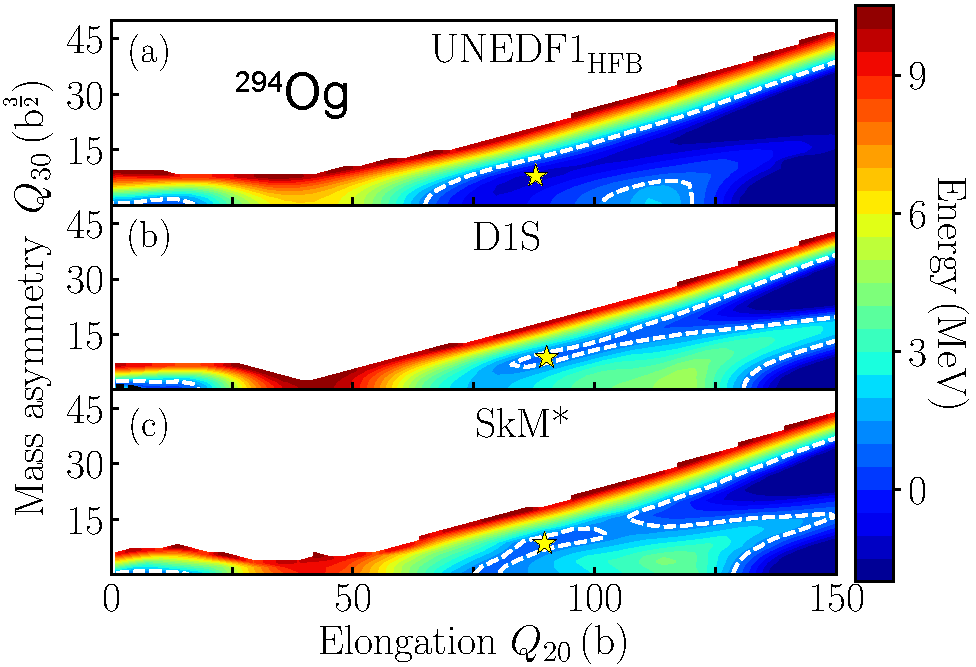
\includegraphics[width=0.7\linewidth]{TeX_files/294Og_three_PES}
	\caption[PES comparison for $^{294}$Og using EDFs {\hfb}, D1S, and SkM*.]{Comparison of the PESs for \Og{} in the $(Q_{20},Q_{30})$ collective plane obtained in \hfb{} (a), D1S (b), and SkM* (c) EDFs. The ground-state energy $E_{gs}$ is normalized to zero. The dotted line in each figure corresponds to $E_0-E_{gs}=1$\,MeV, which was used to determine the inner and outer turning points. The local energy minima at large deformations are marked by stars.}
	\label{fig:294ogthreepes}
\end{figure}

%% This passage is lifted straight from the paper, FYI
But there are  differences as well, such as the height of the first saddle point, the depth of the highly-asymmetric fission valley, and the height of the ridge  separating the two fission valleys. As a result, the outer turning points are pushed to larger elongations in D1S and SkM* as compared to \hfb{}. These differences in the PES topology strongly affect the predicted spontaneous fission half-lives $\tau_\mathrm{SF}$, which in the case of \hfb{}, SkM* and D1S are $9.1\times10^{-9}\,$s, $4.0\times10^{-5}\,$s and $3.2\times10^{-2}\,$s, respectively (see also \cite{Staszczak2013,Baran2015} for a detailed discussion of half-lives). These large variations of $\tau_\mathrm{SF}$ reflect the well-known exponential sensitivity of spontaneous fission half-lives to changes in the quantities entering the collective action \eqref{eq:action}. The $\tau_\mathrm{SF}$ predictions of \hfb{} and, to a lesser degree,  SkM* are incompatible with experiment, as $^{294}$Og  is known to  decay by $\alpha$-decay with a half-life of 0.58\,ms \cite{Brewer2018}. This observation could in fact also apply to the D1S results, since the D1S calculations were performed in a smaller collective space leading to overestimation of the half-lives \cite{Giuliani2014,Sadhukhan2014}. It is to be noted that while half-lives are very sensitive to details of the calculations, the models used here are very consistent with each other and with experiment when it comes to global observables, such as alpha-decay energies, deformations, and radii \cite{Heenen2015,Giuliani2019}. As demonstrated below in Figure \ref{fig:294og3yields}, spontaneous-fission mass and charge yields are also robustly predicted.
%% End of lifted passage

\begin{figure}
	\centering
	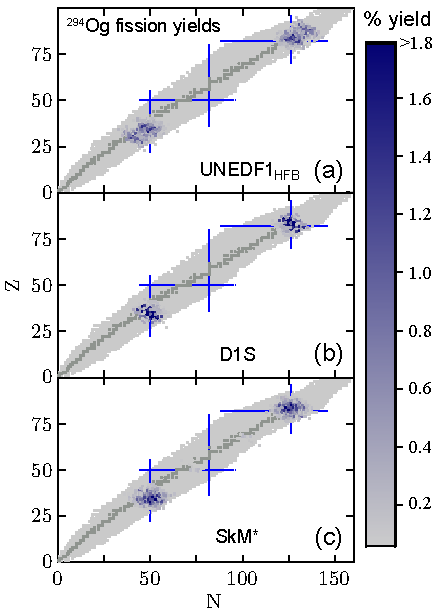
\includegraphics[width=0.9\linewidth]{TeX_files/294Og_3yields}
	\caption[N-Z fission fragment yields from $^{294}$Og]{Fission fragment distributions for \Og{} obtained in \hfb{} (a), D1S (b), and SkM* (c) EDFs using the non-perturbative cranking ATDHFB inertia and  the baseline  dissipation tensor $\mathbf{\eta}_0$. Known isotopes are marked in grey \cite{NUDAT}. Magic numbers 50, 82, and 126 are indicated by dotted lines.}
	\label{fig:294og3yields}
\end{figure}

As expected, the yields are peaked in the region of {\Pb} with a sharp fall-off. Likewise, the projected distributions onto the mass and charge axes shows a clear preference for cluster emission, as seen in the top panels of Figure \ref{fig:294ogcompareall}.

\begin{figure}
	\centering
	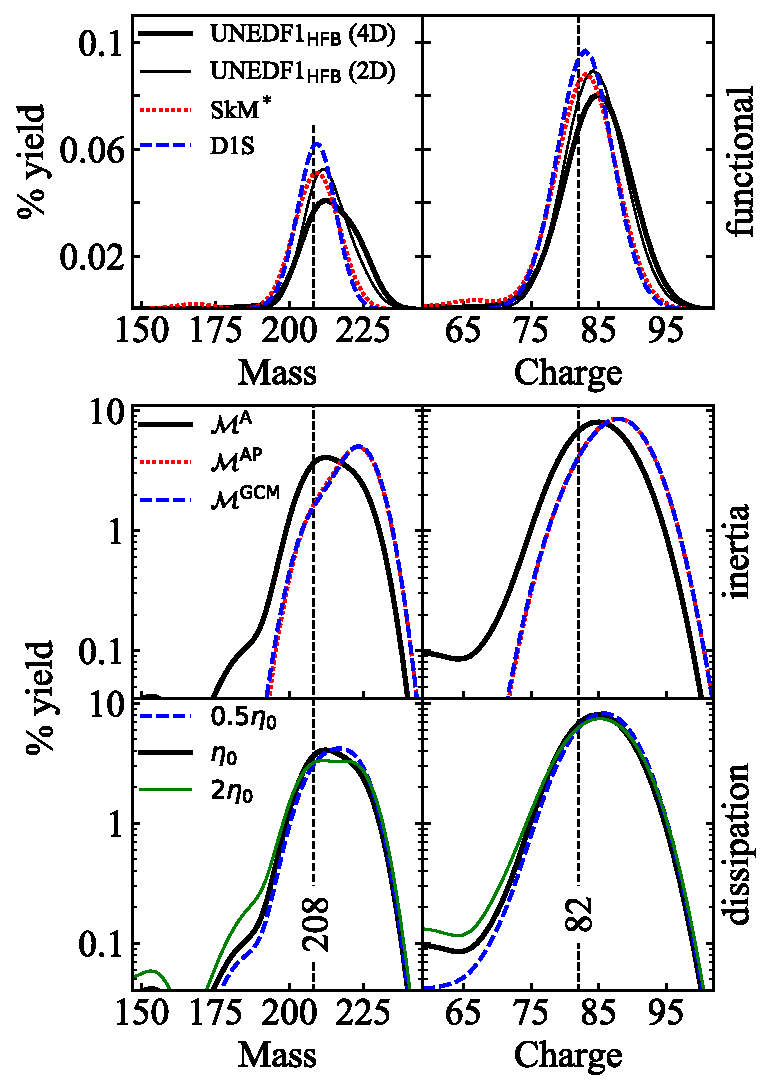
\includegraphics[width=0.7\linewidth]{TeX_files/294Og_compare_all}
	\caption[$^{294}$Og heavy fragment masses and charges.]{Upper panel: Predicted heavy fragment mass (left) and charge (right) yields of \Og{} using different functionals (top, linear scale). Bottom panels: collective inertias and dissipation tensor strengths (in logarithmic scale). The baseline calculation was performed using the \hfb{} functional in a 4D space with non-perturbative cranking ATDHFB inertia and dissipation tensor strength $\mathbf{\eta}_0$.}
	\label{fig:294ogcompareall}
\end{figure}

As discussed in Chapter \ref{chap:Model}, the collective inertia can also have a large impact on the fission dynamics. Using the {\hfb} functional, we compared our result with the non-perturbative cranking ATDHFB inertia {\MATDHF} to the perturbative ATDHFB {\MATDHFp} (which appears smoothed-out compared to {\MATDHF}) and perturbative GCM {\MGCMp} (which is smooth and also lower in magnitude than {\MATDHF} or {\MATDHFp} by roughly a factor of 1.5), which are often easier to use for large-scale calculations. The result, shown in the middle panels of Figure \ref{fig:294ogcompareall}, show that the distribution has shifted slightly, but that {\MATDHFp} and {\MGCMp} give identical, or nearly-identical results. The smoothness of the perturbative inertias apparently allow fluctuations to drive the system to more extreme fragment configurations. This suggests that the magnitude of the inertia matters less than the topography for computing fission yields (though we note that this would not be true for calculating half-lives, which depend exponentially on the magnitude of the inertia).

We also vary the strength of fluctuations by adjusting the parameter $\mathbf{\eta}$. Our starting point $\mathbf{\eta}_0$ is taken from reference \cite{Sadhukhan2016}, where it was obtained by adjusting $\mathbf{\eta}$ to match the experimental fragment distribution of $^{294}$Pu. Shown in the bottom panel of Figure \ref{fig:294ogcompareall}, we find that fluctuations do not affect the peak of the distribution, consistent with the results of Refs. \cite{Randrup2011,Sierk2017,Sadhukhan2017}. The primary effect is in the tails.

\begin{figure}
	\centering
	\includegraphics[width=0.9\linewidth]{TeX_files/294Og_locali}
	\caption[Nucleon localization visualization of $^{294}$Og prefragment formation.]{Nucleon localization functions for several deformed configurations of {\Og}. For comparison, localizations are shown for the fragments {\Pb} and {\Kr} on the left side of each subplot. The configurations shown correspond to Fig. 1 from the paper, with multipole moments $(Q_{20}, Q_{30})=$ (a) (75\,b, 0); (b) (120\,b, 17\,$\mathrm{b}^\frac{3}{2}$); (c) (140\,b, 24\,$\mathrm{b}^\frac{3}{2}$); and (d) (264\,b, 60\,$\mathrm{b}^\frac{3}{2}$).}
	\label{fig:294oglocali}
\end{figure}



\section{$^{294}$Og}

However, although various attempts have been made to demonstrate the validity of this assumption, our work represents the first published instance of a 4D potential energy surface calculated self-consistently. Furthermore, given the recent demonstration of the importance of pairing correlations as a collective ``coordinate'' of the system, ours will feature pairing as part of the collective space, and its impact compared to other collective coordinates will be evaluated.

We used 30 harmonic oscillator shells and 1500 states

\subsection{Cluster Decay}

Experimental instances of super-asymmetric fission:
M. G. Itkis 1985, Z Phys A 320 - no assessment of the cause of highly-asymmetric fission, but likely related to 132Sn (there nuclei would tend to fission symmetrically, but with a slight bump around mass A=140-145)
D. Rochmann Nucl Phys A 735 (2004) - driven by shell structure of lighter fragments
I M Itkis, J Phys Conf Ser 515 (2014) 012008 - cluster radiation by another name

AKA “Lead Radioactivity” sometimes in the literature




\subsection{Competition with Alpha Decay or Half-lives}

%Alex Brown has something: PRC 46, 2, 811-814 (1992) https://link.aps.org/doi/10.1103/PhysRevC.46.811
%Ion’s is in Rom Journ. Phys. 62, 303 (2017) http://www.nipne.ro/rjp/2017_62_7-8/RomJPhys.62.303.pdf
%Roderick Clark: https://journals.aps.org/prc/abstract/10.1103/PhysRevC.97.024333
%Chinese review paper on alpha decay models: https://journals.aps.org/prc/abstract/10.1103/PhysRevC.92.064301

\cite{Poenaru2011, Poenaru2012} - In this paper they propose changing/extending the concept of Heavy Particle Radioactivity or Cluster Radioactivity. Also they apply some model to HPR/CR in SHE.


\section{Method}

% Just say in the methods chapter that ``Our calculations were performed within the framework of nuclear density functional theory using Skyrme energy density functionals, unless otherwise stated \dots We tested this with a variety of inputs, including different functionals, inertias, dissipations, etc. For details of the calculation, see \verb|the paper|.'' I think you can describe the functionals and the inertias here, but don't describe the basis, for instance. What about the collective space? Is it worth showing a figure with the inertias? It's not a bad idea, IF you can make it presentable. You also have that figure showing the 1D barrier using 2D vs. 4D, static vs. dynamic data.

Our calculations were performed within the framework of nuclear density functional theory using Skyrme and Gogny energy density functionals. In the Skyrme case, the parameterization UNEDF1-HFB \cite{Schunck2015} was used, and pairing correlations were described using a density dependent pairing interaction. To assure convergence despite the high density of states, the DFT solver HFODD was used with 30 harmonic oscillator shells and 1500 states allowed in the calculation. Calculations were performed in a 4D collective space consisting of 3 shape coordinates, $(q_{20}, q_{30}, q_{22})$, and, given the importance of dynamic pairing fluctuations demonstrated in \cite{Sadhukhan2014}, $\lambda_2$. To demonstrate model independence, another set of calculations was performed using the Gogny energy density functional D1M in the two-dimensional collective space described by coordinates $(q_{20},q_{30})$.

It is seen in many models that introducing triaxiality as a degree of freedom can often be energetically-favorable, sometimes lowering saddle points by as much as 3 MeV; however, dynamic calculations in which the collective inertia is considered together with the potential energy surface have found that dynamical pathways usually tend to tunnel through barriers rather than break axial symmetry. This competition was explored for SHE in \cite{Gherghescu1999}, with the conclusion that triaxiality plays a fairly insignificant role in determining the half-life of elements below $Z=120$. However, another recent paper (https://arxiv.org/abs/1803.04616v2) suggests that triaxiality might significantly lower the second barrier. Regardless, we included $q_{22}$ in our calculations. It may also be the case that isotopes which are oblate-deformed in their ground state may pass through triaxial configurations on their way to greater elongations.

\section{Experimental efforts to find cluster emission in $^{294}$Og}
Perhaps the biggest uncertainty we'll see, or the biggest deviation from experiment, will be the distribution width. That's because we rather arbitrarily used $\sigma_A=6, \sigma_Z=4$. The values used in 240Pu were 3 and 2, but the $Q_N$ value they used was quite a bit smaller too. Since we had a much larger $Q_N$ cutoff, we needed to account for larger particle number fluctuations. But these numbers were just kind of arbitrary. I'm not too worried about this because the peak is the part that matters, and we clearly saw a peak at the cluster location.

They found 3 (and possibly 4) instances in the original Dubna run. Another Og paper (Brewer2018) has a similar decay chain but a shorter half-life ($\sim$0.185 ms); Detected a 10.6 MeV recoil event, followed 78 microseconds later by a second decay event in the same pixel ($\sim$140 MeV), which is a candidate for SF.

\cite{Brewer2018} they've already started looking, and they're building a new detector that might be able to see it better.